\documentclass{msuphddissertation}
\usepackage{amsmath}
\usepackage{amsfonts}
\usepackage{graphicx}
%\usepackage{hyperref}
\usepackage{enumitem}
\usepackage{minibox}
\usepackage{color}
\usepackage{siunitx}\sisetup{per-mode=symbol}
%\usepackage{tabularx}
\usepackage{listings}

%
%	FRONT
%

\author{Michael J. Obsniuk}
\title{Identifying Computational Practices in Introductory Physics}
\unit{Physics --- Doctor of Philosophy}

\begin{document}

%\maketitlepage

%\begin{abstract}
%Abstract.
%\end{abstract}

\TOC
%\LOT
%\LOF

\newpage
\pagenumbering{arabic}
\begin{doublespace}

%
%	INTRODUCTION (VERY HIGH LEVEL)
%

\chapter{Introduction}

%Computers have revolutionized the way that we do and teach physics \cite{AAPT2016}.
Computers continue to revolutionize the way that we do and teach science.  

\section{Computation is important}

Computation is important as both a research tool and a pedagogical tool.

\subsection{As a research tool}

%Computation is important as a skill in both industry and academia \cite{Chonacky2008}.
Computation is increasingly being referred to as the third leg of modern physics, along with experiment and theory.  Its utility in solving complicated problems (e.g., predicting chaotic or non-linear motion) that cannot currently be solved analytically makes it indispensable in many field, from physics to chemistry to biology to engineering.

\subsection{As a pedagogical tool}

%The use of computation at the introductory level is of great interest as a pedagogical tool \cite{Chabay2008,Kohlmyer2005,Caballero2014,Weatherford2011,Lunk2012}.
Sherwood developed and maintained VPython until it turned in Glowscript.  VPython was expressly designed to engage students with computational modeling and the three-dimensional visualization that are characteristic to it.

Chabay et al. have studied computation involving VPython in introductory physics classrooms from a number of different lenses.  These lenses range from investigating difficulties that students run into while computationally modeling, to investigating how to be incorporate computation into the classroom, to investigating how students are thinking computationally.

%There are still many unanswered questions.
Although much work has been done around computation at the introductory level, there are still many unanswered or only partially answered questions.

\section{Computational thinking}

%DC: I would want to make sure this piece goes into detail about computational thinking and how it is defined with different examples (not just J. Wing, but how other people are talking about it). Then, I think making the argument that it's needed in physics specifically (here's there's lots from my own writing, from AAPT's document, and others). I could see this being a few pages (3 or so). The step to make will be how to take that general talk and then say, well this needs to be in the introductory course (there's some of that argument in my papers and in the AAPT computation document). You can provide the overview of this argument here and then offer more detail in the next chapter.

%Computational thinking has recently been defined as one of the fundamental science and engineering practices \cite{NGSS2012}.
%Computational thinking involves thinking abstractly and algorithmically, and is pervasive \cite{Wing2008, Bundy2007}.
Computational thinking is a term that has become increasingly popular since its introduction in the early 1980s.  This term, although frequently used today, is difficult to concisely explain.  Even within the fields of education and computer science, many different viewpoints exist on the topic, and the corresponding definitions are just as varied \cite{Grover2013}.  However, many of these definitions share one fundamental characteristic: solving complex problems through abstraction and analytic thinking with the aid of computer algorithms.

Seymour Papert first introduced computational thinking in terms of students actively constructing knowledge (constructionism) through the production of an artifact (i.e., a computer program).  However, Papert does not initially attempt to define computational thinking.  Rather, he comments that attempts to integrate computational thinking into everyday life have failed because of the insufficient definition of computational thinking.  He optimistically claims that more attempts to define computational thinking will be made and eventually the ``pieces will come together \cite{Papert1981}.''  Papert would later go on to say that computational thinking involves ``forging new ideas'' that are both ``accessible and powerful \cite{Papert1996}.''

Building on Papert, Jeanette Wing defines computational thinking in terms of taking advantage of the processing power of modern computers with the addition of human creativity.  This echoes the core sentiments expressed by Papert: Using human creativity to forge new ideas that are computationally powerful.  Wing is careful to remind readers that computational thinking is a fundamental skill for everyone, not just computer scientists \cite{Wing2008}.

Further elaboration by Alfred Aho points out that the process of finding the right tool for the right job is a clear indicator of computational thinking.  Mathematical abstraction (modeling) is at the heart of computational thinking, and be able to choose between competing abstractions (models) is of critical importance \cite{Aho2012}.  Aho points out that although there are many useful definitions of computational thinking within computer science, new domains of investigation (e.g., introductory physics) require definitions of their own.

Most recently, the Next Generation Science Standards (NGSS) laid out a framework for identifying computational thinking in K-12 settings.  As early as the fifth grade students are expected to be able to think computationally.  They describe computational thinking, at this level, in terms of analyzing data and comparing approaches.  By the time students reach middle school, computational thinking advances to analyzing large data sets and generating explanations.  Finally, in high school, computational thinking expands to constructing computational models and using them to answer questions \cite{NGSS2012}.  Clearly, computational thinking is a complicated concept which requires substantial explanation.

Experts in the field still have a ways to go when it comes to clearly defining computational thinking within physics education.  However defined, though, this type of abstract and algorithmic thinking is pervasive -- it extends beyond computer science into fields from geology to astronomy, and even beyond STEM \cite{Bundy2007}.  It is becoming increasingly clear that ``computational thinking is a fundamental skill for everyone, not just computer scientists \cite{Wing2006}.'' 

%Solving complex/realistic introductory physics problems requires thinking abstractly and algorithmically \cite{Caballero, AAPT2016}.
One such domain of investigation that could benefit from a clear definition of computational thinking is that of introductory physics.  Many realistic physics problems require thinking abstractly and the computational power of computers (i.e., non-linear forces in Newton's second law).  This combination of abstract and algorithmic thinking (computational thinking) is the ``heart'' of the ``computational physics approach'' to solving problems \cite{AAPT2016}.  This approach relies heavily on computational thinking as it relates to a particular tool and on both technical and physics computational skills.  The AAPT defines 3 technical skills and 7 physics skills. {\bf DC: I think that you can expand on this in Ch 2. Include the table and discuss it.}

Many of the physics skills defined by the AAPT involve modeling and the modeling process.  Computational modeling is a powerful problem solving tool.  Research shows that computational modeling can be successfully incorporated into the (middle-divison) physics classroom \cite{Caballero2011}.  There are a number of common mistakes students make when solving a Newtonian gravitational problem.  We should encourage students to synthesize both analytic and computational skills \cite{Caballero2014}. {\bf DC: I think you can expand on the prior work that studies computation in physics courses in Ch 2. There's also a number of references that you can use to describe the integration of computation into physics courses. They should appear here.}

Other research on (high school) computational modeling has focused on success.  Students' ability to adapt to novel problems seems to rest on the ability to synthesize physics and computational skills \cite{Aiken2012}.  The ability of students to understand the iterative process, that is characteristic of computation, plays a crucial role in the ability to construct novel computational force models.
%Therefore, it is important to encourage computational thinking in introductory physics courses.

Therefore, it is important to encourage computational thinking in introductory physics courses. {\bf DC: I'm not sure how this follows. I want a little more of making an argument. You are describing what folks have done or said, but I want you to have a point from each of these that supports this statement.}

\section{Computational physics practices}

%DC: I think this is a reasonable section to drill down into the argument that we need to define, observe, and encourage computational physics practices if we are going to engage in computational thinking. You have the good set of topic sentences here, but I would want to make sure that it's a bit expanded on here. I think it's ok again to provide overview with references as your background will provide more.

% 1: Practices are a combination of both knowledge and skill \cite{NGSS2013}.
The efficient construction of domain specific knowledge by students has always been one of the ultimate goals of physics education research.  The fundamental concepts, ideas, and theories of introductory physics are the foundation for all inquiry in not just the field of physics, but in many related disciplines (e.g., chemistry and engineering).  However, there is more to being a productive member of the scientific community than just amassing a collection of facts -- it is important that this knowledge be applied in some practical way (e.g., utilizing Newton's second law to numerically predict the trajectory of a rocket).  For this reason, the NGSS has broadly defined scientific practices as a combination of both knowledge and skill ``to emphasize that engaging in scientific investigation requires not only skill but also knowledge that is specific to each practice \cite{NGSS2013}.''  %(DC: I'm not sure that I agree with this definition. Taking from NGSS they are more the actions of science.) 
{\bf DC: This is a good paragraph}

% 2: A taxonomy of general computational practices indicative of computational thinking has been defined \cite{Weintrop2015}.
Given the recent interest in scientific practices, and computational thinking more specifically, a taxonomy of the computational practices indicative of computational thinking has been defined \cite{Weintrop2015}.  This taxonomy, comprised of twenty-two individual yet inter-related practices, fitting into four different categories, is meant to help guide instructors and researchers as they attempt to teach and better understand computational thinking in science classrooms.  Each practice, according to the taxonomy, is defined broadly so as to be applicable to a wide range of science classrooms.

% 3: It is important that we identify (through observation) the set of computational practices that are common to computational introductory physics and encourage them.
% 4: It is important that we understand the knowledge and skills that each computational practice requires.
However, the broad definitions that make the taxonomy widely applicable also leave it relatively vague and difficult to apply to any particular situation.  Reducing the vagueness and difficulty of applying this taxonomy to a specific domain of inquiry (i.e., introductory physics) is a challenging but important task.  Having a taxonomy that is both precise and easy to apply will provide a solid foundation for instructors to generate/validate computational problems and for researchers to analyze the learning process.  Accordingly, it is important that we identify, through direct observation, the set of computational practices that are common to computational introductory physics.  This involves not only identifying the practices, but also the underlying knowledge and skills. {\bf DC: I think this is where you want to say, and this is what this thesis is about: In Ch 2 we blah blah, and in 3 we blah blah blah, etc.}

%
%	BACKGROUND (VERY DETAILED)
%

\chapter{Background} %	VERY DETAILED
\section{Historical and Recent comp. research}
\section{Methods for my research}
\section{Framework}

%
%	CONTEXT (P3)
%

\chapter{Context}
%	Take P-cubed paper and re-write parts focusing on computation.
%	How HAVE we incorporated computational thinking and practices into the course design.
\section{Learning Goals}\label{sec:goals}

${\rm P}^{3}$ uses a number of learning goals to direct pedagogy.  These goals have been generated from two broad categories of focus: the practices we expect students to engage in and the content we hold them responsible for.  Within each of these two broad categories the focus is further broken down into two sub-categories: the fundamental physics principles and the computational implementation of those principles.

\subsection{Practices}

A selection of the scientific practices which we have developed learning goals around are enumerated in no particular order below:  \begin{enumerate}
\item[P1.] developing and using models,
\item[P2.] planning and carrying out investigations,
\item[P3.] analyzing and interpreting data,
%\item using mathematics and computational thinking,
\item[P4.] constructing explanations,
\item[P5.] and engaging in argument from evidence.
%\item and obtaining, evaluating, and communicating information.
\end{enumerate}  These scientific practices were used to inform not only the shared learning goals but also the materials (i.e., projects, exams, homework) we use to achieve those goals.

One of the scientific practices used heavily on both analytic and computation days is that of (P1) developing and using models.  Whether those models be mathematical or computational, we expect students to not only work together in groups to develop the model, but also to utilize that model in further investigations.  As an example, this scientific practice was used to inform the learning goals of:  {\quote Collect, analyze, and evaluate data to explain the motion of objects and the responsible interactions\endquote} \noindent and {\quote Evaluate the applicability/limitations of models and the validity of predictions for different types of motion.
\endquote}  \noindent This type of scientific practice (P1) and the associated learning goals were further used to generate the type of in-class project explicated in Sec.~\ref{sec:example}.

\subsection{Content}

Within the content of ${\rm P}^{3}$ are many ideas that we expect students to grapple with both individually and within their group.  A selection of the previously mentioned sub-categories that we focus on are enumerated below.  The first focus is on the fundamental physics principles: \begin{enumerate}
\item[F1.] macroscopic phenomena are the result of atomic interactions,
\item[F2.] forces external to a system can change the system's momentum,
\item[F3.] and work done on or by a system and heat exchanged with the system's surroundings can change the system's energy.
%\item and left to it's own devices, a system will evolve toward the most common macrostate,
\end{enumerate} The second focus is on the computational implementation of those principles, which takes full advantage of the power of computation: \begin{enumerate}
\item[C1.] computation can be used to predict the otherwise intractable dynamics of real-world phenomena,
\item[C2.] and computation can be used to generate dynamic and graphic representations of real-world phenomena.
\end{enumerate}  Each of these sub-categories of focus were similarly used to inform the shared learning goals and materials used in ${\rm P}^{3}$.

\subsubsection{Physics}

One such learning goal, which focuses on the fact that (F2) forces external to a system can change the system's momentum, is presented to the students as follows: {\quote Apply the momentum principle ($\Delta\vec{p}=\vec{F}_{\rm net}\Delta t;\,d\vec{p}=\vec{F}_{\rm net}dt$) analytically to predict the motion or determine the properties of motion/net force acting on a single-particle system where the net force is a constant vector (e.g., due to the near Earth gravitational force).\endquote} \noindent This goal focuses on the application of a fundamental physics principle (\textit{the Momentum Principle}, $\vec{p}_f = \vec{p}_i + \vec{F}_{\rm net}dt$) in order for students to better understand the dynamics of motion.  This type of reasoning is used extensively in parts A and B of the type of in-class project described in Sec.~\ref{sec:example}.

\subsubsection{Computation}

The computational implementation of the above learning goal which focuses on how (C1) computation can be used to predict the otherwise intractable dynamics of a real-world system is presented to the students in the following way: {\quote Apply the momentum principle ($\Delta\vec{p}=\vec{F}_{\rm net}\Delta t;\,d\vec{p}=\vec{F}_{\rm net}dt$) iteratively/computationally to predict the motion or determine the properties of motion/net force acting on a single-particle system where the net force is not constant (e.g., due to spring-like restoring forces or dissipative drag forces).\endquote} \noindent This goal also focuses on the application of the Momentum Principle, yet takes full advantage of the computational power afforded to the students.  This affordance shows up in the incorporation of a velocity dependent force as described in part C of the in-class project described in Sec.~\ref{sec:example}.

%
%	EXAMPLE PROBLEM
%

\section{Example Project}\label{sec:example}

In order to best illustrate the scientific practices students engage with in ${\rm P}^{3}$, we present a typical problem requiring both analytical and computational techniques over the course of a week (two in-class meetings).  During the second week of class, students are learning how to predict the motion of point particle systems using Newton's Second Law (\textit{the Momentum Principle}, $\vec{p}_f = \vec{p}_i + \vec{F}_{\rm net}dt$) in a project called Escape from Ice Station McMurdo.

\begin{figure}
\centering
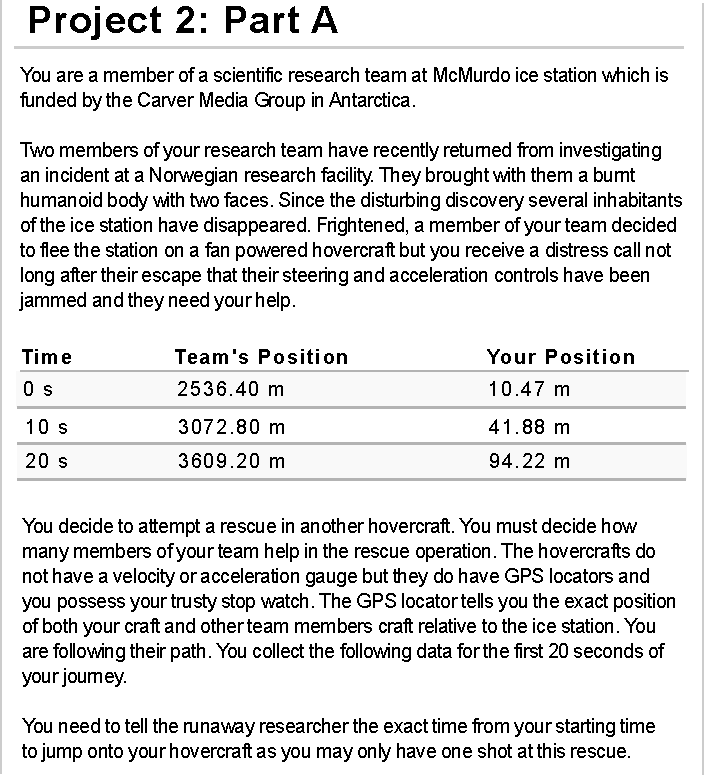
\includegraphics[scale=1]{./images/parta.pdf}
\caption{The first part of a project where students are asked to model the motion of an object given position vs time data.}\label{fig:p2pa}
\end{figure}

In the first part of this three-part problem (Fig.~\ref{fig:p2pa}), students work with position vs time data to model analytically the motion of two hovercrafts as they race across an ice field -- determining the net force from this data and using appropriate models (constant velocity vs constant force) to predict when the hovercrafts will be at the same location.  In the second part of Escape from McMurdo (Fig.~\ref{fig:p2pb}), students find that the controls of both hovercrafts are frozen and they are heading towards a cliff.  They must determine which hovercraft to board in order to survive the fall (there's a salty unfrozen pool at a specific distance from the bottom of the cliff).  The generality and ubiquity of the Momentum Principle is highlighted in the third part of Escape from McMurdo (Fig.~\ref{fig:p2pc}) where the students computationally model the motion of the hovercrafts including air drag. 

\begin{figure}
\centering
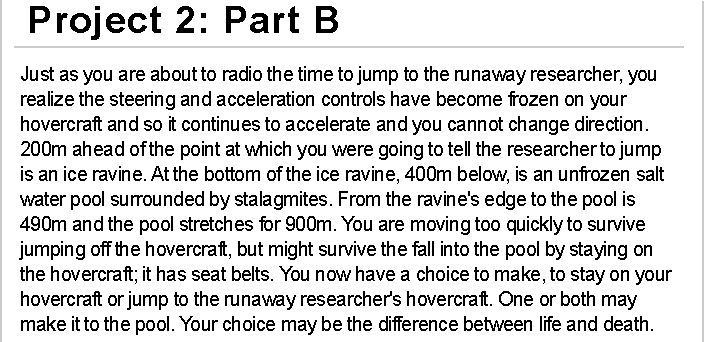
\includegraphics[width=1\linewidth]{./images/partb.pdf}
\caption{The second part of a project where students are asked to model the motion of an object under free-fall conditions.}\label{fig:p2pb}
\end{figure}

\begin{figure}
\centering
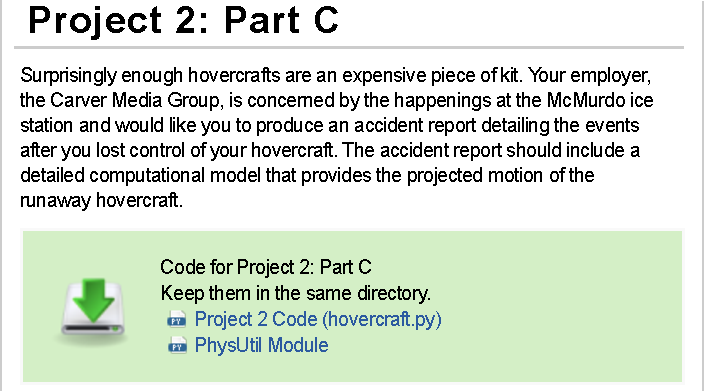
\includegraphics[width=1\linewidth]{./images/partc.pdf}
\caption{The third part of a project where students are asked to model the motion of an object computationally.}\label{fig:p2pc}
\end{figure}

As written above, the Momentum Principle can be used iteratively (through Euler-Cromer integration) to predict the motion of most systems accurately.\cite{Cromer:1981vm}  It turns out both hovercrafts will land safely when modeled without air drag, but students are told that one hovercraft crashes (it lands short). They must file an accident report, which includes a simulation of the accident, to explain how the accident occurred.

Given the complexity of the problems in ${\rm P}^{3}$, a number of different learning scaffolds have been put into place.  These scaffolds are meant to support the students in not only the physics concepts they must use, but also in the scientific practices that they must engage in.  Below, we expound on four such learning scaffolds.

%
%	LEARNING SCAFFOLDS
%

\section{Learning Scaffolds}\label{sec:scaffolds}

\subsection{Modeling Scaffolds}

\subsubsection{The Four Quadrants}

To scaffold the modeling process (Fig.~\ref{fig:modelingprocess}), we have introduced a conceptual tool -- the Four Quadrants.  The Four Quadrants provide a designated location for students to record, reference, and update collectively agreed upon information during the modeling process.  In a sense, the Four Quadrants form the basis of the model, and we provide a designated white board to each group for just this purpose.  Using the Four Quadrants, 
\begin{itemize}[noitemsep,nolistsep]
\item students identify the {\bf Facts}, which are presented in the problem statement;
\item they determine what is {\bf Lacking} from the information they have or can obtain easily;
\item they discuss and negotiate the {\bf Assumptions \& Approximations} they are making; and
\item they provide {\bf Representations} of the problem, which may include diagrams, graphs, or equations.
\end{itemize}

The Four Quadrants are displayed so that not only each member of a group can easily see and modify the agreed upon information, but also so that a group's tutor can easily ``ping'' the group to see where they are in the solution process.  That is, without needing to disrupt the solution process, a tutor can get a well-rounded idea of what the group is thinking and where the group is heading.  This is particularly useful as many tutors are working with multiple groups at any given time.

\subsubsection{Minimal Working Programs}

Many problems in ${\rm P}^{3}$ require the computational modeling of motion and the generation of dynamic plots.  To keep up with the increasing complexity of the problems, students must learn to write VPython code.  However, less than \SI{10}{\percent} of students taking ${\rm P}^{3}$ have any significant computational experience.  We have extended the work of Weatherford\cite{weatherford2011student} and Lunk,\cite{lunk2012framework} who introduced the concept of ``Minimal Working Programs'' (MWPs) to scaffold student sense-making about computing, and to develop a unique, group-oriented, inquiry-based instructional model for computation.  This use of MWPs not only encourages sense-making, but also helps to assuage the anxiety many students have about engaging in computation for the first time.  In this way, we further scaffold the (computational) modeling process.

\begin{figure}
\centering
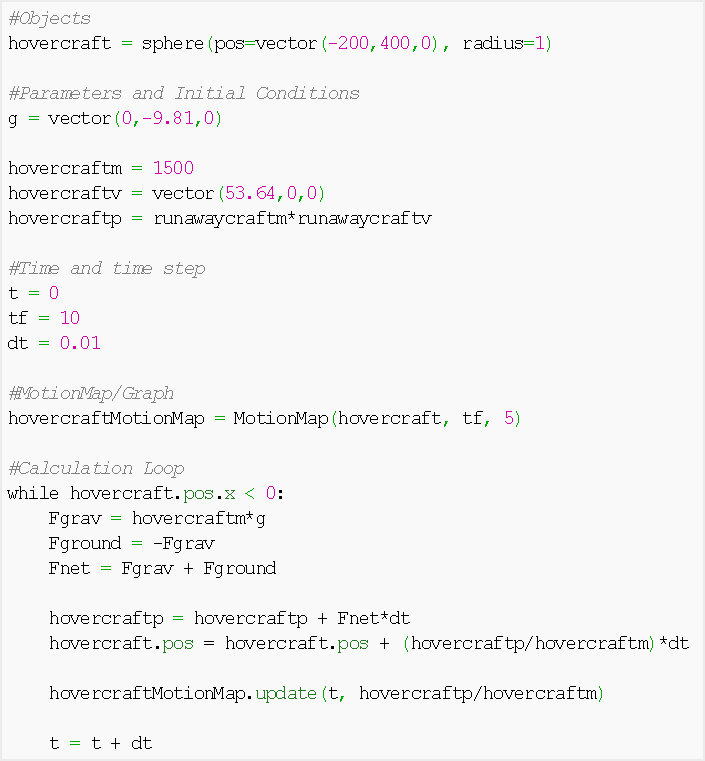
\includegraphics[width=1\linewidth]{./images/code.pdf}\vspace{0.1in}
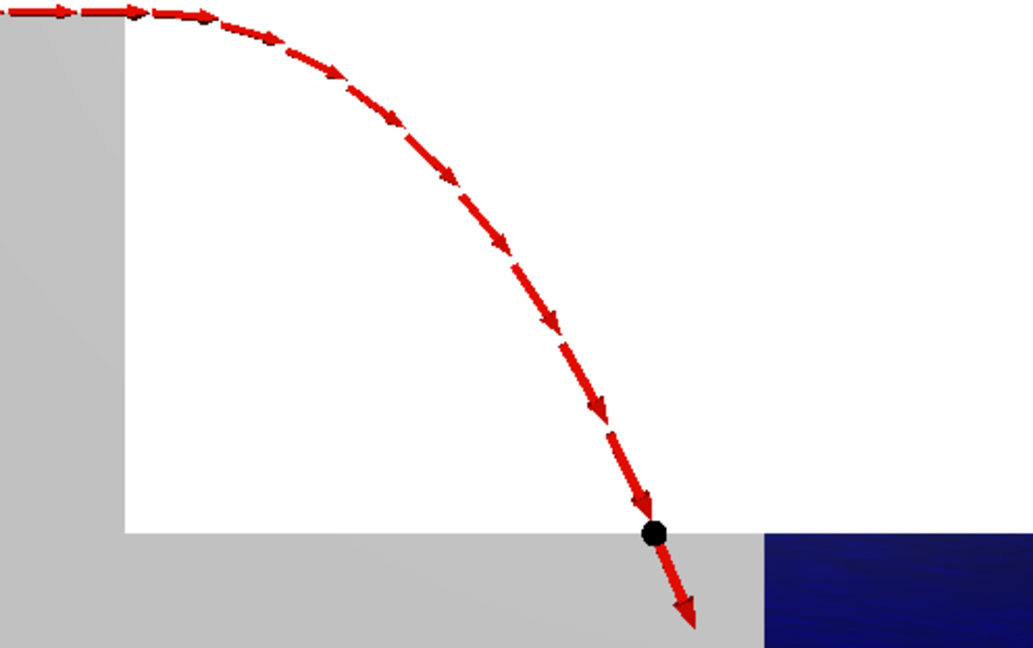
\includegraphics[width=1\linewidth]{./images/visual.pdf}
\caption{Minimally working program that students are provided with for the hovercraft project (top), and a snapshot of the visualization for a completed version of the code (bottom).}\label{fig:code}
\end{figure}

In ${\rm P}^{3}$, students are given no explicit instruction on VPython.  Rather, on computational days, students are provided with a MWP that already predicts the motion of some aspect of the problem (e.g., the motion of a hovercraft up to a certain point on a cliff, as seen in Fig.~\ref{fig:code}).  This experience is similar to receiving ``user-developed'' code from a colleague and extending it to a new situation -- a common practice in science and engineering labs.  By engaging in discussion and negotiation -- two essential science and engineering experiences -- students develop an understanding of what the program is doing and how it is doing it.  They then use that understanding to modify/write additional program statements to model the situation in question.  As a result of this instruction, students having no prior experience with computational modeling are able to write essential elements of the VPython code needed to model novel situations.

We further scaffold this process by providing students with comments -- the gray ``hash-tagged'' (\#) statements in Fig.~\ref{fig:code} that are used consistently and repeatedly in each computational modeling problem.  This common thread throughout MWPs helps to orient the student across many instances of computational motion problems.  Typically, the number of additional program statements students will write is less than 10; they are focused on the core aspects needed to model the system (i.e., motion prediction and visualization).

For example, in the code appearing in Fig.~\ref{fig:code}, students would write several additional lines of code to model the falling hovercraft.  This includes writing a second {\tt while}~loop that stops once the vertical position of the hovercraft coincides with the water, representing force calculations for the air drag and gravitational force in VPython code, and implementing the motion prediction algorithm that performs the appropriate Euler step. 

\subsection{Content Scaffolds}

\subsubsection{Conceptual Homework}

Much of the student experience in ${\rm P}^{3}$ is working through complex problems that require discussion and negotiation among group members to develop a complete solution.  To support student success when solving these problems in class, we ``prime the pump'' with pre-class readings/video lectures and homework.  Each week, students read online lecture notes, watch short video lectures, and solve conceptual and reasoning-focused homework on-line, which are meant to scaffold students' conceptual understanding that they will bring to bear in class that week.

Often, solutions to computational problems can take many syntactical forms, while the underlying computational algorithm is identical.  That is, VPython has a number of functions to simplify the typing/reasoning that any group of students must undertake.  For example, as shown in Fig.~\ref{fig:compHW}, when taking the magnitude of a vector \texttt{object.pos}, two possible methods accomplish the same goal:  the ``manual'' way of explicitly squaring, summing, and square rooting the vector componentits \texttt{sqrt(object.pos.x**2+obj.pos.y**2+obj.pos.z**2)} and the VPython short-cut way of \texttt{mag(obj.pos)}.  Given the diverse computational background of students in ${\rm P}^{3}$, we highlight these differences/similarities in the pre-homework to scaffold the discussion and solution process.

\begin{figure}
\centering
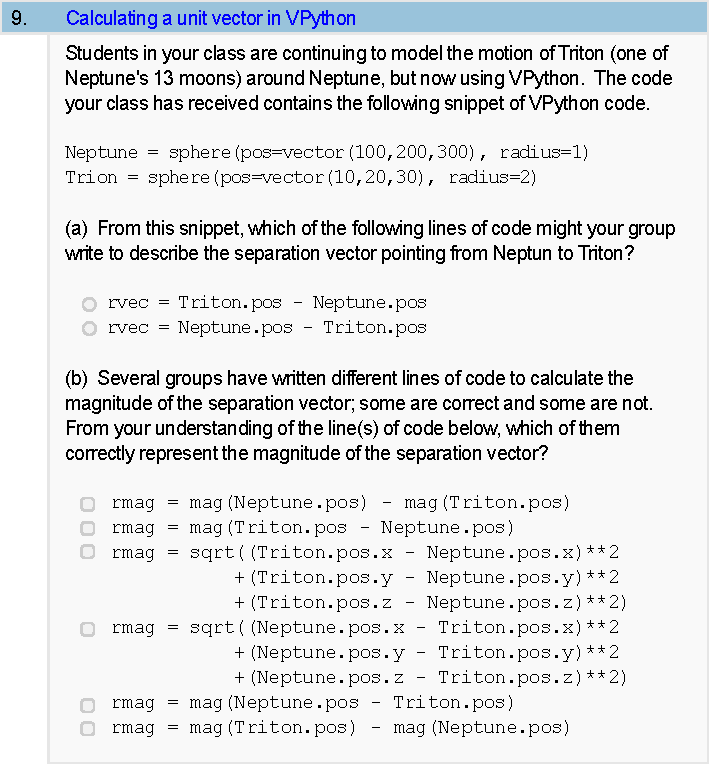
\includegraphics[width=1\linewidth]{./images/comphw.pdf}
\caption{Computational pre-homework problem focusing on the different ways to construct a unit vector in VPython.}\label{fig:compHW}
\end{figure}

After each pair of weekly class meetings, students complete additional conceptual and reasoning-focused homework as well as more typical back-of-the-book style problems.  These are designed to provide a wrap-up of the week's material and to encourage the students to take full advantage of the opportunity to engage in group discussion and sense making in class.

\subsubsection{Tutor Questions}

With such open ended projects as shown in Sec.~\ref{sec:example}, there are many possible solution paths that lead to the same answer, and the course staff works to encourage any solution path that utilizes the concepts and ideas being focused on for that week.  In order to ensure a group's understanding of the content being focused on, we have introduced a compilation of questions which are meant to confront common misconceptions and to test for basic understanding, as exemplified in Fig.~\ref{fig:tutorq}.

\begin{figure}
\centering
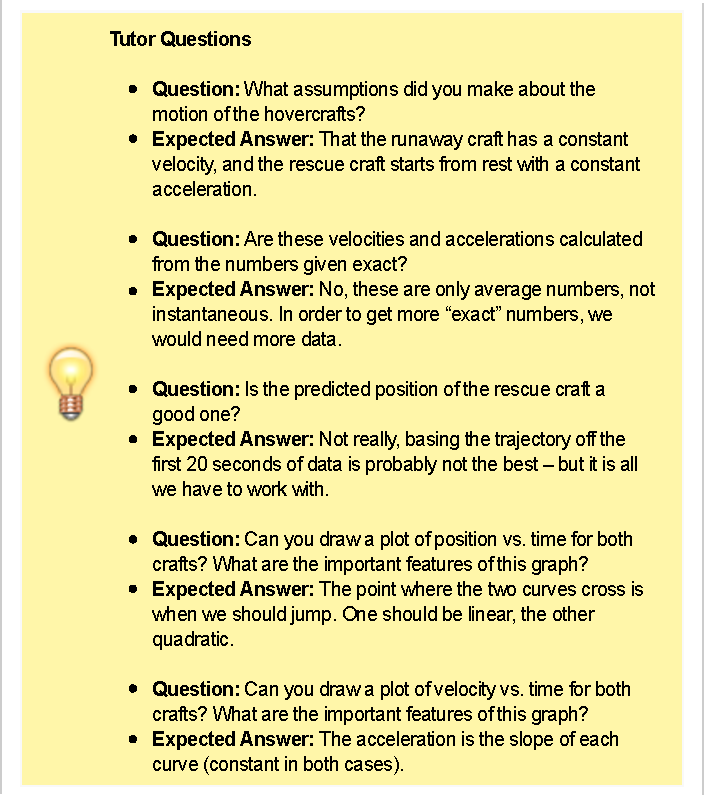
\includegraphics[width=1\linewidth]{./images/tutorq.pdf}
\caption{A selection of the tutor questions that are asked during the hovercraft problem.}\label{fig:tutorq}
\end{figure}

The generation of these tutor questions is a continuous and iterative process.  Initially, questions are generated by consulting with the literature and by ``testing'' the project.  As the projects are delivered to students in-class, new solution paths inevitably arise with unique lines of reasoning.  These new lines of reasoning generate new tutor questions, which are added to the compilation.  We aim to compile a robust set of tutor questions spanning many different solution paths.

The nature of the pre-class homework mentioned previously is largely conceptual, and often requires an answer of the free-response type.  Given that these homeworks are delivered using an electronic web-based system, answers may be easily collected and analyzed by course staff to highlight any particularly difficult topics.  These topics may then be used by the tutors as ``just-in-time'' style talking points during class.  In this way, the tutor is not only informed of which topics to check for understanding on, but also which students may need a little extra attention.

%
%	MOTIVATION
%

%	Add in debugging paper and expand on it for the motivation.
\chapter{Motivation for identifying broader practices}

\section{Debugging}

\subsection{Introduction}

Since the development of reasonably affordable and fast computers, educators have argued for their inclusion in the classroom as both a learning aid and a tool.\cite{DiSess1986,Shecker1993}  With the recent development of high-level programming languages capable of quickly rendering three-dimensional real-world simulations, the argument for the inclusion of computers in the classroom has not only persisted, but has grown.\cite{Chonacky2008}  Well into the 21$^{\rm st}$ century, with its prevalence in modern physics research, we see computation being increasingly referred to as the ``third pillar'' of physics -- along with the more canonical pillars of theoretical and experimental physics.\cite{Chabay2008}

One physics curriculum that includes a computational element is Matter \& Interactions (M\&I).  The M\&I curriculum differs from a traditional one not only through the inclusion of computation (VPython), but also through its emphasis on fundamental physics principles and the addition of a microscopic view of matter.\cite{Chabay2004,Chabay1999}  Recent work\cite{Kohlmyer2005,Caballero2012} involving students' use of VPython with the M\&I curriculum has begun to analyze the patterns seen in implementing and assessing the use of computation in introductory physics courses.

However, numerous questions remain unanswered regarding the processes observed while groups of students work together to model real world phenomena computationally.  We extend our research to a novel implementation of M\&I with an emphasis on computation in a group setting, called Projects and Practices in Physics (${\rm P}^{3}$), where students negotiate meaning in small groups, develop a shared vision for their group's approach, and employ science practices to navigate complex physics problems successfully.  Borrowing from the literature of computer science education research,\cite{McCauley2008} we use the notion of computational debugging in a physics context to help uncover the salient practices unique to computational physics problems.

In this paper, we present a case study of a group of students immersed in this ${\rm P}^{3}$ environment solving a computational problem.  This problem requires the translation of a number of fundamental physics principles into computer code.  Our analysis consists of qualitative observations in an attempt to describe, rather than generalize, the computational interactions, debugging strategies, and learning opportunities unique to this novel environment.

\subsection{Assumptions}

In an increasingly technological world, we have at our disposal computers well suited for the most procedural and tedious, yet indispensable of STEM tasks.  Accordingly, in ${\rm P}^{3}$, we treat the computer as an indispensable \emph{modern tool} with which students must familiarize themselves.  In spite of the fact that modern computers \emph{take} meaningful direction quite well, they do not yet posses the faculty to \emph{generate} meaningful direction on their own.  This necessitates a human factor, in which groups of students must leverage their understanding of fundamental physical principles to model real world phenomena computationally (i.e., generate meaningful direction to a computer).

We focus our research on the interactions between group and computer to begin to understand the ways in which computation can influence learning.  Particularly, we are interested in the interactions occurring simultaneously with social exchanges of fundamental physics principles (FPPs) specific to the present task (e.g., discussing $d\mathbf{r}=\mathbf{v}\,dt$ on a motion task) and the display of desirable strategies (e.g., divide-and-conquer), as illustrated in Fig.~\ref{interactions}.  These group-computer interactions vary in form, from the more interactional process of actively sifting through lines of code, to the less interactional process of observing a three-dimensional visual display -- in this work, the more the student interacts with lines of code, the more interactional.

\begin{figure}
\caption{A group of students interacting with VPython where social exchanges focus on FPPs and desirable strategies are being exhibited.}
\resizebox{0.9\columnwidth}{!}{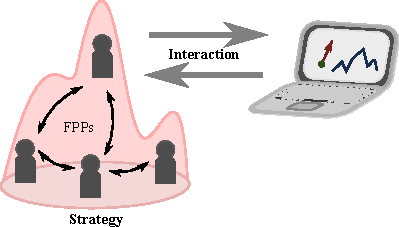
\includegraphics{./images/interactions.pdf}}
\label{interactions}
\end{figure}

One previously defined computational interaction that reinforces desirable strategies,\cite{Murphy2008} borrowing from computer science education research, is the process of debugging.  Computer science defines debugging as a process that comes after testing \emph{syntactically} correct code where programmers ``find out exactly where the error is and how to fix it.''\cite{McCauley2008}  Given the generic nature of the application of computation in computer science environments (e.g., data sorting, poker statistics, or ``Hello, World!'' tasks), we expect to see unique strategies specific to a computational \emph{physics} environment.  Thus, we extend this notion of computer science debugging into a physics context to help uncover the strategies employed while groups of students debug \emph{fundamentally} correct code that produces unexpected physical results.

\subsection{Data}

In Fall 2014, ${\rm P}^{3}$ was run at Michigan State University in the Physics Department.  It was this first semester where we collected \emph{in situ} data using three sets of video camera, microphone, and laptop with screencasting software to document three different groups each week.  From the subset of this data containing computational problems, we \emph{purposefully sampled} a particularly interesting group in terms of their computational interactions, as identified by their instructor.  That is, we chose our case study not based on generalizability, but rather on the group's receptive and engaging nature with the project as an \emph{extreme case}.\cite{Flyvbjerg2006}

The project that the selected group worked on for this study consists of creating a computational model to simulate the geosynchronous orbit of a satellite around Earth.  In order to generate a simulation that produced the desired output, the group had to incorporate a position dependent Newtonian gravitational force and the update of momentum, using realistic numerical values.  The appropriate numerical values are Googleable, though instructors encouraged groups to solve for them analytically.

This study focuses on one group in the fourth week of class (the fourth computational problem seen) consisting of four individuals: Students A, B, C, and D.  The group had primary interaction with one assigned instructor.  Broadly, we see a 50/50 split on gender, with one ESL international student.  Student A had the most programming experience out of the group.  It is through the audiovisual and screencast documentation of this group's interaction with each other and with the technology available that we began our analysis.

\subsection{Analysis}

To focus in on the group's successful physics debugging occurring over the $\SI{2}{\hour}$ class period, we needed to identify phases in time when the group had recognized and resolved a physics bug.  These two phases in time, \emph{bug recognition} and \emph{bug resolution} are the necessary limits on either side of the process of \emph{physics debugging}, as represented in Fig.~\ref{phases}.  We identified these two bounding phases at around $\SI{60(5)}{\minute}$ into the problem, and further examined the process of debugging in-between.  That is, we focused on the crucial moments surrounding the final modifications that took the code from producing unexpected output to expected output.

\begin{figure}
\caption{The debugging process necessarily corresponds to a phase beset on either side by the phases of recognition and resolution.  Note the absence of a vertical scale, as the vertical separation merely acts to distinguish phases.}
\resizebox{0.9\columnwidth}{!}{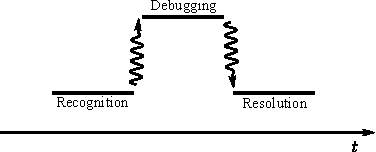
\includegraphics{./images/phases.pdf}}
\label{phases}
\end{figure}

\subsubsection{Bug recognition}

At around $\SI{55}{\minute}$ into the problem, following an intervention from their instructor, the group began to indicate that they were at an impasse:  \begin{verbatim}
    SB:  We're stuck.
    SD:  Yeah...
\end{verbatim}  The simulation clearly displayed the trajectory of the satellite falling into the Earth -- not the geosynchronous orbit they expected.  This impasse was matched with an indication that they believed the FPPs necessary to model this real world phenomenon were incorporated successfully into the code:  \begin{verbatim}
    SB:  And it's gonna be something really 
         dumb too.
    SA:  That's the thing like, I don't think 
         it's a problem with our understanding 
         of physics, it's a problem with our 
         understanding of Python.
\end{verbatim}  Instead of attributing the unexpected output with a mistake in their understanding or encoding of FPPs, they instead seemed to place blame on the computational aspect of the task.

During this initial phase, we see a clear indication that the group has recognized a bug -- there is an unidentified error in the code, which must be found and fixed:  \begin{verbatim}
    SA:  I don't know what needs to change 
         here...
    SD:  I mean, that means we could have 
         like anything wrong really.
\end{verbatim}  Although they have identified the existence of the bug, they still are not sure how to fix it -- this necessitates the process of debugging.

\subsubsection{Physics debugging}

Within the previously identified phase of bug recognition, the group developed a clear and primary task: figure out exactly how to remove the bug.  Eventually, following a little off-topic discussion, the group accepted that in order to produce a simulation that generates the correct output, they must once again delve into the code to check every line:  \begin{verbatim}
    SA:  ...I'm just trying to break it down 
         as much as possible so that we can 
         find any mistakes.
\end{verbatim}  In this way, the group not only determined the correctness of lines of code that have been added/modified, but also examined the relationships \emph{between} those lines.

For example, the group began by confirming the correctness of the form of one such line of code:  \begin{verbatim}
    SA:  Final momentum equals initial momentum
         plus net forces times delta t.  True?
    SC:  Yeah...
    SB:  Yes.
    SA:  O.K.  That's exactly what we have 
         here.  So this is not the problem.
         This is right.
    SD:  Yeah.
\end{verbatim}  That is, Student A \emph{(i)} read aloud and wrote down the line of code $\vec{p}_{f}=\vec{p}_{i}+\vec{F}_{\rm net}\Delta t$ while the entire group confirmed on its correct form.  This written line was then boxed, and was shortly followed up \emph{(ii)} with a similar confirmation of the line $\vec{r}_{f}=\vec{r}_{i}+\vec{v}\Delta t$ that immediately prompted \emph{(iii)} the confirmation of $\vec{v}=\vec{p}/m$.  Thus, not only do we see the group determining the correctness of added/modified lines of code as in \emph{(i)}--\emph{(iii)}, we further see confirmation with the links \emph{between} those lines, as in the velocity from \emph{(ii)} being updated through the momentum from \emph{(i)} given their relationship from \emph{(iii)}.

The group ran through these types of confirmations with FFPs rapidly over the span of a few minutes.  Once the group had confirmed all the added/modified lines of code to their satisfaction, the discussion quieted down.  The FPPs were winnowed from the discussion, and after a little more off-topic discussion we find them seeking help from the instructor:  \begin{verbatim}
    SD:  Maybe we should just stare at him 
         until he comes help us...
\end{verbatim} Suddenly, a haphazard change to the code:  \begin{verbatim}
    SA:  You know what, I'm gonna try 
         something.
\end{verbatim} where Student A changed the order of magnitude of the initial momentum a few times.  This modification eventually resulted in a simulation that produced the correct output.

\subsubsection{Bug resolution}

At $\SI{65}{\minute}$ into the problem, Student A changed the order of magnitude of the momentum one final time, which produced something \emph{closer} to the output that they expected:  \begin{verbatim}
    SA:  Oh wait... Oh god...
    SD:  Is it working?
\end{verbatim}  The satellite now elliptically orbited the Earth.  This marks the end of the debugging phase and the beginning of the resolution phase -- the bug had successfully been found and remedied.  Given that the only line of code modified to produce this change was the initial momentum, they began to rethink the problem:  \begin{verbatim}
    SD:  I think that is the issue is that 
         we don't have the initial momentum...
    SA:  ...momentum correct?
\end{verbatim}  That is to say, the group pursued the issue of determining the correct initial momentum with the added insight gained through debugging fundamentally correct VPython code.

\subsection{Discussion}

To summarize, in analyzing this particular group, we first identified the two phases in time when the group had recognized and resolved (see Fig.~\ref{phases}) a physics bug.  We then necessarily identified the phase in-between as the process of physics debugging in ${\rm P}^{3}$, where the fundamentally correct code was taken from producing unexpected output to producing expected output.  Given our assumption that the process of computer science debugging encourages desirable strategies, we then began to analyze this process of physics debugging further for strategies unique to ${\rm P}^{3}$.

Given the actions exhibited during the debugging phase, we can separate them into two distinct parts: a more strategic part and a less strategic part, as shown in Fig.~\ref{strategy}.  The group initially gave indication that they were working in a considerate, thorough, and consistent manner, which we classify as more strategic.  This is contrasted by the later indications of more haphazard actions, which we classify as less strategic.  These are the two physics debugging strategies that, together, led to the resolution of the bug in this context.

\begin{figure}
%\source{Source}
\caption{Physics debugging phase consisting of more and less strategic strategies specific to our case study.  Note the absence of a vertical scale, as the vertical separation merely acts to distinguish phases.}
\resizebox{0.9\columnwidth}{!}{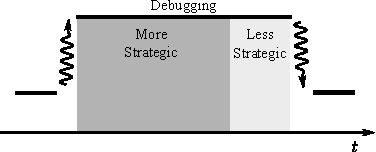
\includegraphics{./images/strategy.pdf}}
\label{strategy}
\end{figure}

The more strategic strategy was exhibited through the confirmation of individual FPPs as well as their relation to others.  Not only did the group confirm through discussion, they simultaneously wrote, boxed, and referenced equations in the code -- this helped to reduce the number of FPPs they needed to cognitively juggle at any given time.\cite{Redish2003}  This confirmation of FPPs through discussion presented a great learning opportunity for the entire group, where creative and conceptual differences could be jointly ironed-out.  Accordingly, we tentatively refer to this strategy as \textbf{self-consistency}.

Although the resolution of the bug might not be tied directly to this self-consistency, that does not negate the learning opportunities afforded to the group along the way.  Specifically, we saw the group double-checking every fundamental idea used and, possibly more importantly, the links between those ideas.  Being physically self-consistent in this manner is a desired strategy in ${\rm P}^{3}$.

The less strategic strategy was exhibited during the haphazard changes to the initial momentum.  These changes to the code that eventually resolved the bug, though one of the benefits of computation (i.e., the immediacy of feedback coupled with the undo function), could have been more thoughtful.  A deeper understanding of the physics or computation could have tipped the group off to the fact that the initial momentum was too small.  Again, this does not negate the learning opportunities afforded to the group through this less strategic strategy, which resembles that of ``productive messing about.''\cite{Podolefsky2012}  Accordingly, we tentatively refer to this strategy as \textbf{play}.

Both of these strategies identified here, self-consistency and play, hold implications for the learning opportunities afforded to groups.  More research is needed to dissect these learning opportunities and to deepen our understanding of the strategies themselves.
\vspace*{0.2in}
\subsection{Conclusion}

This case study has described two strategies (one more and one less strategic) employed by a group of students in a physics course where students develop computational models using VPython while negotiating meaning of fundamental physics principles. These strategies arose through the group's process of debugging a fundamentally correct program that modeled a geosynchronous orbit. The additional data we have collected around students' use of computation is rich, and further research is needed to advance the depth and breadth of our understanding of the myriad of ways in which students might debug computational models in physics courses.

\section{Phenomenography}

\section{Task Analysis}

\subsection{Introduction}\label{intro}

Given the ever increasing complexity of modern scientific problems, computation is essential practice that physics and engineering majors must learn \cite{chonacky,AAPT}.  However, integrating computation into physics courses does not come without its challenges for both instructors and students \cite{chabay}.  Currently, researchers understand little about the challenges that students face when connecting computational practices with physical concepts.  Thus, it is important that we not only identify these challenges, but also investigate the way in which students overcome them.

The study presented in this paper takes place in a practice focused group learning environment at Michigan State University called P-cubed \cite{pcubed}.  In this environment students solve analytical and computational mechanics problems (using VPython) in small groups. For computational problems, we make use of minimally working programs -- incomplete but functional programs that encourage students to focus on the fundamental physics of the phenomena, rather than getting bogged down in code syntax and program structure \cite{weather}.

As part of a larger project investigating the challenges that students experience with computation in introductory physics classrooms, we conducted a task analysis on a computational problem that we have observed students struggling to complete over the last several semesters.  This gravitational orbit problem is delivered in the third week of class and requires groups to construct a position dependent Newtonian gravitational force that is fully generalizable (i.e., capable of handling elliptical orbits).  We used task analysis to identify specific sub-tasks that students must complete in order to solve the problem. We then identified clips from in-class video where students are engaging in those tasks in order to describe the different lines of reasoning that students are using while solving the problem. Due to the limit of space, our analysis presented here is restricted to the construction of the direction of the gravitational force.

\subsection{Methods}\label{methods}

Our primary source of data comes from in-class video of students developing a VPython program to model a gravitational orbit. In order to focus our analysis on specific challenges students demonstrate while working this problem, we developed a framework for analyzing this problem by performing an expert task analysis on the problem.  A task analysis consists of breaking a complex ``task'' (e.g., modeling a gravitational system) down into related ``sub-tasks'' (e.g., determine the direction of the force). We aim to identify somewhat more manageable steps that must be taken in order to complete the overall task \cite{catra}.
%Our expert analysis included input from three instructors with experience in teaching introductory physics with MWPs in a PBL-style classroom, ensuring a robust and thorough analysis.

The task analysis of this problem was initially constructed by a single content expert. After the first iteration it was presented to additional experts. Through this discussion, it became clear that the construction of the position dependent Newtonian gravitational force in code is a multi-step procedure involving a number of different sub-tasks. The task analysis was iteratively refined through this process until all experts agreed that the sub-tasks were sufficiently described to be useful in video analysis. At the same time, targeted pre-class homework problems were developed to help scaffold students overcoming what we perceived to be challenges based on the task analysis.  In doing so, we attempted to place (most) students in the Zone of Proximal Development (ZPD) \cite{vyg}. For example, the pre-class homework problems shown in Fig.~\ref{unit_hw} were developed to facilitate student understanding of the unit vector of a separation vector between two objects prior to working the computational problem.

\begin{table}[hb]
\caption{Some of the necessary steps that must be taken when constructing a Newtonian gravitational force in code.  Each step is associated with the construction/modification of a line of code.\label{tab1}}
\begin{tabular}{ll}
\textbf{Step (Sub-Task)} & \textbf{Associated Code} \\\hline
Construct separation vector & \begin{lstlisting}
sep = obj2.pos
\end{lstlisting}\\
between interacting objects & \begin{lstlisting}
         - obj1.pos
\end{lstlisting}\\\hline
Construct the unit vector & \begin{lstlisting}
usep = sep/mag(sep)
\end{lstlisting}\\\hline
Construct the net force & \begin{lstlisting}
Fnet = -G*m1*m2*usep
\end{lstlisting}\\
vector & \begin{lstlisting}
         /mag(sep)**2
\end{lstlisting}\\\hline
Integrate the net force over & \begin{lstlisting}
obj.p = obj.p + Fnet*dt
\end{lstlisting}\\
time into momentum & \\
\end{tabular}
\end{table}

With an agreed upon task analysis, we further focused our video analysis on the sub-tasks that were closely related to the construction of the position dependent Newtonian gravitational force (see Table.~\ref{tab1}).  In order to identify when groups were actually engaging in these sub-tasks, we analyzed groups on two levels: their \textit{speech}, including any and all words or utterances, and the associated \textit{visuals}, including any drawings, writings, lines of code, gestures, or simulation visualizations.  Theses two levels were then used to better understand how students overcome the challenges associated with the problem.

\subsection{Analysis}

There were a number of challenging tasks undertaken by students that were identified in the video.  For the sake of clarity within the allotted space, we will focus on one sub-task: the construction of the \textit{direction} of the Newtonian gravitational force in code.  This was one of more challenging sub-tasks with which groups struggled.  It requires the group, depending on how they break the problem down, to:
\begin{enumerate}[nolistsep,noitemsep]
  \item
  define the separation vector between the satellite and the Earth,
  \item construct its unit vector, and
  \item use that unit vector to give a direction to the force.
\end{enumerate}
It is important that all of these definitions be placed in the calculation loop of the MWP given that they must change over (simulated) time.

\begin{figure}[ht]
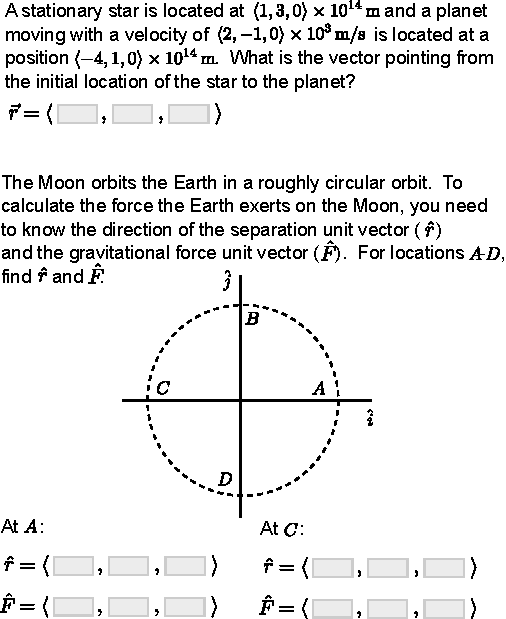
\includegraphics[width=0.8\linewidth]{./images/hw.pdf}
\caption{Pre-class homework problems delivered in the second week of class that are specifically designed to strengthen the connection between a separation vector, its unit vector, and the direction of a force.\label{unit_hw}}
\end{figure}

Below, we present three episodes of three different groups engaging with the problem described in Sec.~\ref{intro}. We have paid particular attention to the lines of reasoning that the students are taking while articulating their solutions.

%
%	Group A
%

\subsubsection{Episode: Group A}

Group A is comprised of Cody, Chuck, Shelley, and Joe.  Group A has an equal gender distribution and Chuck has the most programming experience (and does most of the coding).  This episode begins at around half way into the class after a tutor interaction where the group is dissuaded from using a centripetal form (i.e., $mv^{2}/R$) of the net force.  Rather, they decide to use a Newtonian form (i.e., $F_{\rm G}=Gm_{1}m_{2}/R^{2}$) so that it will be able to handle elliptical orbits.


\vspace*{4pt}
\noindent\textbf{Shelley}: {\it But ummm wait, hold on, remember this?  The uniform circular is equal to the gravity is equal to the net?  So we could just do what you did, except instead of using the uniform circular motion equation we use that gravity equation [points to equation].}\\
\textbf{Joe}: {\it Yeah...}\\
\textbf{Chuck}: {\it Okay, yeah, that sounds good.}
\vspace*{4pt}

However, after coding the magnitude of the Newtonian gravitational force (i.e., \texttt{Fnet = G*mEarth*msat/R**2}) the group is still unsure of how to add in the direction.

\vspace*{4pt}
\noindent\textbf{Chuck}: {\it How do we, okay, how do we define a direction?}\\
\textbf{Cody}: {\it I don't know...}\\
\textbf{Chuck}: {\it Isn't the direction like, okay, so here I'm gonna give like four points on a circle [drawing on whiteboard] so this is the center, and this is a b c and d.  Isn't it always just the position vector of a, so ummm what is it, like satellite dot position minus position dot Earth, and then you can divide that by magnitude?}
\vspace*{4pt}

At this point, the group has worked out a plan to construct a unit vector that can be used to add onto the magnitude of the Newtonian gravitational force to give it the proper direction.  They successfully follow through with this plan after comparing the unit vector at multiple points along a unit circle.

\vspace*{4pt}
\noindent\textbf{Chuck}: {\it Okay, so we're going e minus a, so it's just negative, it's always negative e, right?  What if we pretend it was here, what is it doing, now would it be like, x is point five... I think, okay so, arbitrary like it's not on the circle, so it would be like point five in the x direction, point five in the y direction, and zero in the z direction.  So you're still taking that minus that and the direction would be negative points five negative point five, so I think that would still apply, if we are taking c minus a, and then divide by magnitude, would that make sense?}
\\\textbf{Cody}: {\it So how does that apply to this? How can we apply that concept?}
\vspace*{4pt}

They then construct this in the code taking advantage of the built in \texttt{mag()} function to calculate a magnitude of a vector.\begin{lstlisting}
R = 123
[calculation loop]
    dir = sat.pos/mag(sat.pos)
    Fnet = -G*m1*m2*dir/R**2
\end{lstlisting}

Although the magnitude of the net force is not generalizable enough to handle elliptical orbits at this point (the distance \texttt{R} is defined outside of the calculation loop), they have successfully added in the direction of the Newtonian gravitational force.  It is important to note that Chuck uses a procedure that is very similar to what is required on one of the pre-class homework problems shown in Fig.~\ref{unit_hw}.  In both cases, comparing multiple points along a unit circle can help to develop a sense for the direction of a separation vector and its use in giving a direction to a force.

%
%	Group B
%

\subsubsection{Episode: Group B}

Group B is comprised of Kayla, Jon, Angela, and Alan.  Group B has an equal gender distribution and Alan has the most programming experience.  This episode begins at about a quarter of the way into the class with the group agreeing to use a centripetal form of the gravitational force that they just so happen to have a vector equation for (i.e., $\vec{F}_{\rm net}=mv^{2}\langle\sin\theta,\cos\theta-1\rangle/R\theta$).

\vspace*{4pt}
\noindent\textbf{Kayla}:  {\it So, I have the uniform circular motion up... [scanning notebook] Ummm, magnitude of net force... uniform... Ummm...}\\
\textbf{Alan}:  {\it We should calculate the force, the ``centripetal force'', and then use that number?}\\
\textbf{Kayla}:  {\it Yeah...}\\
\textbf{Alan}:  {\it Sounds good.  What are the equations for that?}\\
\textbf{Kayla}:  {\it Oh wait, hey, look at that, okay, these ones have, they are vector components ummm [writing on whiteboard].}
\vspace*{4pt}

The group is unsure of the validity of the equation that used the satellite's polar angle ($\theta$), and Alan begins to consider how the velocity will have a different direction at various points along a unit circle.

\vspace*{4pt}
\noindent\textbf{Alan}:  {\it So like right here... like we would have a total velocity like going in the x direction or from here in the x direction and then right here going down so now it's all in the y direction there's no x direction, it's like oscillated between the maximums so we could get a rotation... but how do we represent that as a force means it's obvious that they want us to do that so do we...}
\vspace*{4pt}

Immediately, Kayla proposes the equation from her notebook again.  The group is convinced that this equation will lead to the expected oscillation of the direction of the velocity.

\vspace*{4pt}
\noindent\textbf{Kayla}:  {\it Sine and cosine?}\\
\textbf{Alan}: {\it Sine and cosine?}\\
\textbf{Kayla}: {\it If we do sine and cosine, if we do both of them one in the x, one in the y, like this is saying [points to equation], then even if one goes to zero like you were saying then the other one is gonna be close to one and so...}\\
\textbf{Alan}: {\it Do we have our angles to use?}\\
\textbf{Angela}: {\it Ohhh...}\\
\textbf{Alan}: {\it And we have access to angles... because we have access to the time of day.}\\
\textbf{Angela}: {\it That would make sense cause then if you're at some weird angle because like...}\\
\textbf{Kayla}: {\it Yeah...}\\
\textbf{Angela}: {\it Right here one of them is gonna go to one, the other one is gonna go to zero like...}\\
\textbf{Bruce}: {\it Oh my god that's so great, that's perfect, you're totally right.}
\vspace*{4pt}

Indeed, they have all the necessary components needed to quickly construct this calculation in their code (i.e., the angle that the Earth is making).

Although this group is making progress toward a net force that changes with position, they still have several steps to complete this angular calculation.  However, before they can construct any significant piece of code, the group is dissuaded by a learning assistant from using the polar angle of the satellite and are encouraged to use a unit vector in terms of a separation vector vector and its magnitude.  It is important to note that, like Group A,  Group B was also comparing multiple points along a unit circle in order to develop a sense for the way in which a physical quantity (i.e., the velocity of the satellite) needs to change direction.

%
%	GROUP C
%

\subsubsection{Episode: Group C}

Group C is comprised of Tori, Natalia, Connor, and Alex.  Group C has an equal gender distribution, with one ESL student, and Connor has the most programming experience.  The episode begins at around three-quarters of the way into the problem.  We can see Connor comparing the ``radius'' of the satellite's orbit at two different locations, one point on the perimeter of a unit circle and one point beyond it.

\vspace*{4pt}
\noindent\textbf{Connor}: {\it Well, if we start like that [drawing on whiteboard], but then we move over say here where it isn't equal radius, then our y value changes right?}\\
\textbf{Tori}: {\it Yes.}
\vspace*{4pt}

This immediately turns into Tori reasoning out the way to calculate a separation vector between two objects.

\vspace*{4pt}
\noindent\textbf{Tori}: {\it So ummm, I thought, so the Earth is at zero zero zero, so in all of our homeworks, what we did was, the Earth is zero zero zero and then we have a position of the satellite at ummm...}\\
\textbf{Connor}: {\it 4210...}\\
\textbf{Tori}: {\it Yeah, like that zero, zero.  So when you subtract this, it is like, you know what I mean?  We need one going from here to there, which would mean that we need to take this one minus this one so this one, minus that, which is just that, because you're just taking this minus zero.}
\vspace*{4pt}

Again, we see Connor comparing a physical quantity at two different locations, and Tori explicitly references the pre-class homework.

\vspace*{4pt}
\noindent\textbf{Connor:} {\it But then say we are up here [points to whiteboard]...}\\
\textbf{Tori:} {\it Yeah, and I think because in all the homeworks we have done this one was for like, oh, this is from okay a planet to a star, but they never talked about that moving in circular orbit}...
\vspace*{4pt}

This discussion eventually leads to the construction of the net force in code that uses the separation vector between the Earth and the satellite.  \begin{lstlisting}
R = 123
[calculation loop]
    Fnet = -const_G*m1*m2/R**2 * sat.pos
\end{lstlisting}

Although the magnitude of the gravitational force is still incorrect at this point, they have successfully incorporated one of the important components for the direction of the net force in code (i.e., the separation vector \texttt{-sat.pos}).  It is important to note that Tori explicitly reference the pre-class homework problem shown in Fig.~\ref{unit_hw} when reasoning out the direction of the gravitational force.  Also, Connor can be seen running through a very similar process to that of Groups A and B (i.e., comparing physical quantities at different locations).

\subsection{Discussion \& Conclusions}

We have shown the lines of reasoning that three different groups have taken while working to overcome the challenges associated with constructing a position dependent Newtonian gravitational force in VPython code.  Due to the brevity of this paper, we focused on the sub-task of constructing the \textit{direction} of the Newtonian gravitational force.  In our analysis, we saw three separate cases of groups comparing the change in a physical quantity (e.g., the gravitational force or the velocity) at multiple points along and near the perimeter of a unit circle.  In each case, while groups made these comparisons, we also saw them beginning to construct the direction of the Newtonian gravitational force: Groups A and C added in a direction based on a separation vector, and Group B started to add a direction based on a polar angle.

These episodes suggest that the pre-class homeworks shown in Fig.~\ref{unit_hw} are providing appropriate scaffolding for students \cite{vyg}.  Group A explicitly compares the direction of the net force at four different points on the unit circle.  Group B compares the direction of the satellite's momentum at two different points on the unit circle.  Group C compares the distance of the satellite from the origin at two different points on and near the unit circle.  It appears that asking students to solve related yet sufficiently different problems can familiarize students with the important concepts so that they can be extended into novel in-class problems.%  Similar pre-class questions have been used on other computational problems in P-cubed.

%The question of whether and how computation can help to teach physics concepts is still an open one.  Although we have begun to make progress towards a deeper understanding, there is still more to learn about what makes a good pre-class homework question.  Effectively complementing introductory physics with computation is a difficult process, and we believe that the research we have presented here can be used, in part, to ease that process.

In an effort to broaden this investigation, we have begun conducting one-on-one post-class interviews to investigate the qualitatively different ways in which students experience introductory physics with computation.  These interviews show promising descriptions of the reasoning taking place around computational physics tasks.  For example,

\vspace*{4pt}
\noindent\textbf{Ski}: {\it This [gravitational] problem especially showed me why it's important to update the force, the direction of the force. Going into this, I never thought of force, I didn't even know force was a vector. I thought it was a magnitude with a direction... which is a vector. I don't know, I guess that in my head force was positive or negative in direction. This problem definitely helped me to learn that we needed to use the r hat vector... For me, this entire problem was about velocity and the force pointing downwards, but downward changes.}
\vspace*{4pt}

In the future, we aim to synthesize this and other data to form a deeper and broader understanding of how computation can be used in physics courses to help students develop a deeper understanding of physics content and practice.

%
%	IDENTIFYING PRACTICES
%

\chapter{Identifying computational practices}

Our analysis of the in-class group computational problem solving in ${\rm P}^{3}$ can be broken down into a number of different resolutions/scales.  One resolution/scale that we can focus on is the individual group and the different practices that they are engaging in.  Each practice identified within a particular group, as broadly defined in the Weintrop Framework, manifests in multiple possible variations.  The amount of variation observed usually depends not only on the practice (i.e., some practices are generally more diverse/varied than others) but also on the particular group (i.e., some groups engage in more diverse/varied practices).

\section{Specific methods}

\subsection{Transcription}

We transcribe the entire problem solving process that has been captured on video, paying specific attention not only to what the group is saying, but also to what the group is doing (e.g., typing lines of code, gesturing, etc.).  Any lines of code that are typed can be verified by checking against the screencast of the group's laptop.  Any written equations or scratch work can be checked against the overhead camera.  These different sets of data are then used in conjunction while searching for practices. 

It is very rare that we see groups explicitly defining their actions in terms of the language of the framework.  Accordingly, we need to infer what the groups are thinking from the data.

\subsection{Mill's method?}

\section{Findings}

Recall that, according to the framework, each category of practice can be broken down into a number of individual practices.  Each individual practice, further, can be identified in terms of a number of fundamental characteristics.  Depending on the particular situation, some categories show up in the data more often than others.  For example, we expect to see fewer systems thinking practices and more computational modeling practices.  Further, within any category, some individual practices show up in the data more than others.  For example, within the data practices, we expect to see fewer instances of collecting data and more instances of creating data.

Most importantly, within any individual practice, there is a broad set of defining characteristics.  Ideally, each characteristic would be present in some form when its corresponding practice has been identified.  However, each characteristic can be organized in terms of being either necessary or sufficient for the cause.  That is, we need not necessarily observe every characteristic in order to identify a practice according to the framework.

\begin{figure}[ht]\centering
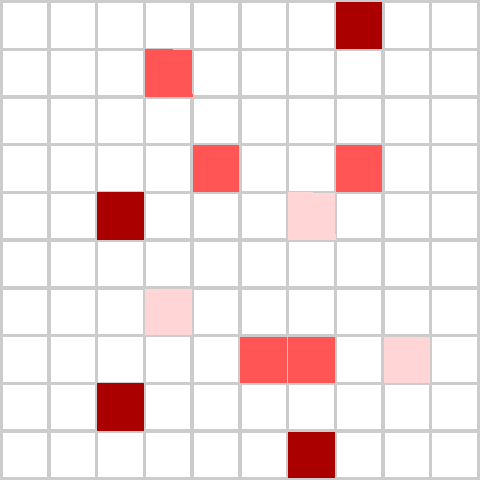
\includegraphics[scale=1]{./images/matrix.pdf}
\caption{A matrix showing the frequency of computational practices across the data set.}
\end{figure}

\subsection{Assessing computational models}

\begin{figure}\centering
  \begin{tabular}{ r | c | c | c | l}
    Excerpt & Model & Phenomenon & Comparison & Assessing computational models \\ \hline
    A.X &   &   &   &   \\
    B.X &   &   &   &   \\
    C.X & * & --  & * & * \\
    D.X  &   &   &   &   \\
    E.X &   &   &   &   \\
    F.X &   &   &   &   \\
    G.X &   &   &   &   \\
    H.X & * & -- & -- & -- \\
    I.X & * & * & * & * \\
  \end{tabular}\caption{A table to look for the possible necessary and sufficient characterstics (Mill's joint method of agreement and difference) for the individual practice of assessing computational models.}
\end{figure}

\subsubsection{Models}

Get rid of these tables.  Not worth the trouble.

\begin{figure}[ht]\centering
  \begin{tabular}{ r | c | c | c | c | c | l }
    Excerpt & A & B & C & D & E & Model \\ \hline
    C.X & -- & --  & * & * & -- & * \\
    H.X & -- & -- & * & -- & * & * \\
    I.X & * & * & -- & * & * & * \\
  \end{tabular}\caption{A table to look for the possible necessary conditions (Mill's method of agreement) for any characteristic -- Mill's method of agreement.}
\end{figure}

\subsubsection{Phenomena}

asd

\subsubsection{Comparisons}

sdf

\subsubsection{Variation}

sdf

%
%	DISCUSSION
%

\chapter{Discussion}

%
%	CONCLUSIONS
%

\chapter{Concluding Remarks}

%
%	APPENDICES
%

\appendices

\chapter{Problem statement?}

\chapter{Transcripts?}

%
%	BIBLIOGRAPHY
%

\end{doublespace}

\bibliography{bibliography}
\bibliographystyle{plain}

\end{document}

%
%	EXTRA
%

%\begin{landscape}
%\thispagestyle{empty}
%\captionof{table}{caption_text}
%\captionof{figure}{caption_text}
%\end{landscape}